\documentclass[12pt,oneside]{fithesis2}


\usepackage[english]{babel}
\usepackage[utf8]{inputenc}
\usepackage{lmodern}
\usepackage[T1]{fontenc}

\usepackage[scaled=0.86]{berasans}
\usepackage[scaled=1.03]{inconsolata}
\usepackage[plainpages=false, pdfpagelabels]{hyperref}

\usepackage{enumitem}
\usepackage{microtype}
\usepackage[top=3.0cm, bottom=3.5cm, left=2.4cm, right=2.4cm]{geometry}	% pc version
%\usepackage[top=3.0cm, bottom=3.5cm, left=2.9cm, right=1.9cm]{geometry}	% print version

\usepackage[backend=biber,style=ieee]{biblatex}
\addbibresource{thesis.bib}

\usepackage{minted}
\setminted{framesep=2mm, frame=lines}

\usepackage{multicol}
\usepackage{subcaption} 

\usepackage{tikz}
\usetikzlibrary{trees,calc,shapes.arrows}


\thesislang{en}
\thesistitle{GPU-based speedup of EACirc project}
\thesissubtitle{Bachelor Thesis}
\thesisstudent{Jiří Novotný}
\thesiswoman{false}
\thesisfaculty{fi}
\thesisyear{Spring 2015}
\thesisadvisor{RNDr. Petr Švenda, Ph.D.}



\newcommand{\todo}{
	%\bigskip
	\noindent
	{\large\color{red}\textbf{TODO}}
	%\bigskip
}


\begin{document}
\FrontMatter
	\ThesisTitlePage
	%\begin{ThesisDeclaration}
	%	\DeclarationText
	%	\AdvisorName
	%\end{ThesisDeclaration}
	%\begin{ThesisThanks}
		%TODO Thesis Thanks
	%\end{ThesisThanks}
	%\begin{ThesisAbstract}
		%TODO Thesis Abstract
	%\end{ThesisAbstract}
	%\begin{ThesisKeyWords}
		%TODO Thesis Keywords
	%\end{ThesisKeyWords}
	\tableofcontents

\MainMatter
\chapter{Introduction}
Random data and the concept of randomness are used in many branches of informatics. However one of the most fundamental usage of these principles is in cryptography and IT security. For instance let there be an communication among several entities. The main content of the communication is mend to stay hidden from the others, thus the communication needs to be encrypted by some chosen encryption protocol. The potential attacker \footnote{The one who wants to know the hidden content of the encrypted communication without permission of legal participants.} could intercept some encrypted messages and subject them to analysis. On the basis of certain traits of the protocol or similarities among individual messages the encryption could be broken and the hidden content of the communication could be read by the attacker. Thus the goal of encryption protocols is that the encrypted messages would not be similar or would not have some characteristic traits. In other words the encrypted messages must look like random data to the attacker. But these constraints are very difficult to provide.

That is why have been created tools to test randomness and thus quality of ciphers. One of these tools is called EACirc and is developed at Faculty of Informatics at Masaryk University in CRoCS laboratory (Centre for Research on Cryptography and Security). It can tell how much are the input data close to a referential random data. \footnote{This is only an approximative explanation. The exact definition and meaning of EACirc results are described in Martin Ukrop's thesis Usage of evolvable circuit for statistical testing of randomness. \cite{ukrop_thesis}} To achieve that it uses raw computation power. But the computations made are not run in parallel and doing that could significantly speed-up the whole process. Faster evaluation could advance capabilities of EACirc and help it to test the randomness in much more detail.

The speed-up of EACirc is achieved with running some chosen computations on a GPU. The GPU must have got a build-in support of a general purpose programming (GPGPU). Such chip can perform not only algorithms used in rendering of computer graphic but also almost every other algorithm that is runnable on a CPU. The main difference against CPU is that the CPU is optimized to minimize latency whereas GPU is optimized to maximize throughput. Latency is a number meaning how much time is going to take a single instruction to load needed data and to execute the instruction. On the other hand throughput is a number meaning how much data the instruction can process per one time unit. \footnote{In current common computation model it is almost impossible to reduce latency together with the growth of throughput on a one device. The more data we load the longer time it takes.} Since some parts of EACirc processes a lot of data with algorithms, which does not need to be optimized for latency \footnote{An algorithm that needs to be optimized for latency in order to maximize performance is that one that has lots of edges in it's control flow graph.}, the usage of GPU's is suitable.

Because GPGPU programming needs a specially enhanced hardware from the manufacturer there are several different solutions on the market. The solution that is used for this thesis is called CUDA \cite{about_cuda} and it's a proprietary technology developed by NVIDIA. \cite{nvidia} The decision to use CUDA was made by my advisor.

Since the performance of GPGPU is dependable on used hardware the achieved speed-up was measured by an experimental method. The benchmarks took place particularly on machines that laboratory of CRoCS is using for own computations and are capable to run a CUDA code.

\medskip

To set the project of EACirc to use the CUDA technology required non-trivial intervention to settings for building the project from the sources aka the makefiles. This intervention would have resulted in a long-term unmaintainable and chaotic project if the previous workflow would have been preserved.  To prevent that the secondary objective of this thesis was to improve the previous build-system of the EACirc project using the open-source CMake \cite{cmake} supportive tool developed by Kitware \cite{kitware} corporation.





\chapter{CUDA}
As stated on the NVIDIA website \cite{about_cuda}, "CUDA is a parallel computing platform and programming model that enables dramatic increases in computing performance by harnessing the power of the graphics processing unit (GPU)." The strengths and weaknesses of GPU lies in it's architecture and in differences from CPU. A GPU that is able to execute CUDA programs is addressed as \emph{CUDA capable device} or simply as the \emph{device}.

\begin{figure}[H]
	\centering
	\includegraphics{figures/gpu-devotes-more-transistors-to-data-processing.png}
	\caption{"The GPU Devotes More Transistors to Data Processing." NVIDA. \cite{cuda_guide}}
	\label{fig:cpu_vs_gpu_arch}
\end{figure}

\noindent
The figure \ref{fig:cpu_vs_gpu_arch} shows a high level view of the CPU and GPU architecture. In both there are the same parts: DRAM, Cache, Control, and ALU. DRAM and Cache are memory chips, the difference is that Cache is much more smaller but significantly faster. The Control unit is responsible mainly for instruction fetching, decoding, etc. ALU is simply a worker that processes the input data. CPU's Control unit and Cache is much more bigger and focuses on flow control and data caching in order to reduce the latency. The GPU's counterparts are simpler but multiplied allowing to focus on data processing (throughput) and data parallelism. It is worth mentioning that the DRAM of a GPU is significantly faster in order to supply enough data to the big number of ALUs and to keep them busy. \footnote{The memory model of GPU is described in section \ref{memory_hiearchy}.}

\begin{figure}[H]
	\centering
	
	\begin{subfigure}[b]{0.45\textwidth}
		\includegraphics[width=\textwidth]{figures/memory-bandwidth.png}
		\caption{"Memory Bandwidth for the CPU and GPU." NVIDIA. \cite{cuda_guide}}
	\end{subfigure}
	\hfill
	\begin{subfigure}[b]{0.45\textwidth}
		\includegraphics[width=\textwidth]{figures/floating-point-operations-per-second.png}
		\caption{"Floating-Point Operations per Second for the CPU and GPU," NVIDIA. \cite{cuda_guide}}
	\end{subfigure}
	
	\caption{The contrast of GPU and CPU performance in throughput}
	\label{fig:cpu_vs_gpu_performance}
\end{figure}

The performance of GPU is mainly measured by two variables: floating point operations per second (FLOPS) and memory bandwidth. The figure \ref{fig:cpu_vs_gpu_performance} shows the theoretical maximum performance on NVIDIA GPU's in contrast to Intel CPU's in terms of throughput.

\section{Architecture of CUDA capable devices}
\label{cuda_architecture}

In both, CPUs and GPUs, DRAM (fig. \ref{fig:cpu_vs_gpu_arch}) is significantly slower than ALU. If an ALU requires some data from DRAM, the ALU must wait hundreds of clock cycles to the data to became available (viz. latency). The waiting is highly ineffective and it is usually solved with executing another thread's instruction which has it's data available. The difference between CPU and GPU is how often is going to happened that an instruction wants data from DRAM.

Today CPUs use SIMD (Single Instruction, Multiple Data) execution model. It processes a vector of data with only one instruction. The data are cached massively to reduce latency\footnote{Data caching is a technique to avoid waiting for data which are stored in a slow storage by introducing memory hierarchy. When data are requested, they are firstly searched for in faster memory. When they are not found (cache miss) then a slower memory is searched as long as they are found. Then they are promoted to the faster memory to become available to subsequent requests (cache hit).} and so the ALU does not need to wait. Thus, if big data are not accessed wrongly, the probability of cache miss is low and switching context to a different thread can be relatively expensive operation. 

The execution model of CUDA is called SIMT (Single Instruction, Multiple Threads). Instead of vector of data, a vector of threads is executed with one instruction simultaneously. The vector of threads resides in one of the control units. Each thread of the execution vector is then mapped to an ALU related to the control unit. Each control unit has it's own cache. Since the cache is smaller, the cache miss is going to happen more often and another vector of threads, which has all its resources available, is executed. The switching of a thread context is done instantly with null overhead.\footnote{The section \ref{memory_hiearchy} describes how is this achieved.} Thus to keep the GPU busy, more threads than is the number of ALUs must be running.

In CUDA terminology the control units are called \emph{Streaming Multiprocessors} (SMs). Each SM has it's own ALUs referred to as \emph{cores}. The single thread vector composes of 32 threads which is called a \emph{warp}.


\section{Thread hierarchy}

The SIMT architecture of GPU is well suited (and designed) for computational problems that can be optimized using data parallelism. Data parallelism is a parallelization technique that divides the input data to the independent parts and executing them separately (but evenly) on parallel computing nodes. The final result is then composed from each sub-result. CUDA platform supports this technique through kernels and thread hierarchy.

In CUDA context a \emph{kernel} is a top-level function that is runnable on CUDA capable devices. It is recommended that the kernel should process only the smallest portion of input data that can be processed separately. For instance, when adding two vectors, the kernel should just add two corresponding scalars of the vector.

For each kernel, that is being run, a separate thread is created on the device. As shown in the figure \ref{fig:grid}, a group of threads is forming a \emph{block} and a group of blocks is forming a \emph{grid}. Each thread has got unique ID dependant on it's position in the block and each block has unique ID dependant on it's position in the grid.\footnote{The grid might have up to 3 dimensions.}

\begin{figure}[H]
	\centering
	\includegraphics{figures/grid-of-thread-blocks.png}
	\caption{"Grid of Thread Blocks." NVIDIA. \cite{cuda_guide}}
	\label{fig:grid}
\end{figure}

\noindent
The dimensions of the grid should correspond to the dimensions of the computational problem. In the example of adding vectors the grid should have same width as the number of scalars in the vector. Since each thread has a unique ID the kernel knows which scalars to and add what is the position of the result in the final vector.

The execution of a single kernel is initiated as soon as the device has enough available resources to run a whole block. This constraint allows that the threads of one block can communicate with each other (viz. section \ref{memory_hiearchy}) and that the computational problem can be scaled across different types of CUDA GPUs disposing other hardware capabilities.\footnote{For instance the number of cores or available memory.} The execution order of the blocks is not defined.

To fully utilize the device the size of the block should be multiple of a warp size\footnote{For current devices the warp size is 32 (viz. section \ref{cuda_architecture}).}. Each block is mapped to a single SM (viz. \ref{cuda_architecture}). On a single SM several blocks may be active, but the exact number is dependant on the GPU hardware parameters. Depending of the number of SMs several block may be run in parallel. This is fully done by the CUDA platform. but the programmer should know these constraints to produce optimized code for each device.

\section{Memory hierarchy} \label{memory_hiearchy}



\section{CUDA capabilities}
\section{Toolkit}
\section{Programming}





\chapter{CMake}
The EACirc sources mainly consists of \emph{C} and \emph{C++} code. The code was divided into reasonably logical sections but the overall structure and concept of the project were monolithic.\footnote{A monolithic binary is an executable that does not need any other dependencies or resources at a runtime. In other words, the binary is independent.} This led to compilation of all sources into one big executable of approximately 9~MB which took some non-trivial time.

On top of this EACirc is developed as a cross-platform application. To provide native builds for each supported platform (Windows \cite{win} and Linux) special makefile or an IDE specific project file were used which described how to build the application. When a change in the build was introduced, e.g. a new source file was added, the change had to be manually implemented to all makefiles to provide consistency. This workflow was not easy to maintain as the violation of these rules could cause an uncomfortable pitfall.

To solve these problems the CMake \cite{cmake} tool was integrated into the project of EACirc along with some changes to the basic structure of EACirc. The CMake tool is developed and maintained by Kitware, Inc. \cite{kitware} as an open-source software. The main purpose of this tool is to provide native builds of cross-platform applications and to minimize the effort to maintain the project.

Although there are many similar tools as CMake and some of them provides better features they are not so widely supported. For instance CMake generates project files for almost every common IDE and some of those IDEs comes with a built-in support for CMake.

\section{CMake toolset}

The CMake is actually a set of several tools that are taking care of building, testing, and deploying a user's \emph{C} or \emph{C++} project. These tools can be installed on Linux, Windows, or MacOSX. The CMake toolkit consists of the main tool \texttt{cmake} and the supportive \texttt{ccmake} (or \texttt{cmake-gui}), \texttt{ctest}, and \texttt{cpack}.

The \texttt{cmake} tool takes a configuration file called \texttt{CMakeLists.txt} distributed with the project source files and generates the platform specific makefiles as an output. Then the user invokes a platform specific tool for building -- usually \texttt{make}, \texttt{ninja} \cite{ninja}, or \texttt{MSBuild}. \cite{msbuild} If the process is successful the native binaries of the project are now made.

The \texttt{ctest} tool provides a simple platform for project testing. If the build is successful the user can run some custom made tests on the binaries.

The \texttt{cpack} tool provides a cross-platform mean to deploy your application on the target system.

The remaining \texttt{ccmake} and \texttt{cmake-gui} are just more convenient ways to use a \texttt{cmake} tool since \texttt{cmake} has only a command line interface. The former provides a TUI\footnote{Text-based user interface (TUI)} and the latter provides GUI\footnote{Graphical user interface (GUI)}.

\section{A closer look at the \texttt{cmake} executable}

The \texttt{cmake} executable is not just a dummy build-system. The process of generating a makefile is quite sophisticated. At first the user chooses the \emph{source directory} and the \emph{build directory}. Then (s)he invokes the \texttt{cmake} command in a \emph{build directory} with appropriate parameters. The subsequent process consists of several phases -- selection of a native build-system (in a CMake terminology referenced as a \emph{generator}), configuration based on a user-specific input, and the own generation of a makefile.\footnote{Note that the exact scheme of this process can differ according to which interface of CMake is used -- i.e. \texttt{cmake}, \texttt{ccmake}, or \texttt{cmake-gui}.}

The \emph{source directory} is simply a directory where the project sources are located and as well as the top-level \texttt{CMakeLists.txt} file which is distributed with the sources. The build directory is an empty user-created directory in which the user wants the binaries to be build.

The selection of the \emph{generator} depends on the user's platform, on the user-installed native build-systems, and on the user's intentions. The generator used on Linux is usually \texttt{make} or \texttt{ninja}. When the user wants to generate project files to a specific IDE, he chooses the appropriate generator -- e.g. Visual Studio 2013 \cite{msvc} on Microsoft Windows \cite{win}. Usually the selection of the appropriate generator is done by CMake automatically.

The subsequent phase is configuration. Here the user specifies variable options for the build that the project supports. For instance some features of the application can be switched on/off or the location of a third party dependencies can be specified. Also the different build configuration can be switched, i.e. release or debug.

If the configuration is all right then the makefile is successfully created in the \emph{build directory}. Then the user just invokes the appropriate tool to execute the makefile and the binaries are build.

It is worth mentioning that the makefile automatically detects any changes made in the \emph{source directory}. So the user invokes the \texttt{cmake} executable just once to generate the makefile or to change the variable options of the build. The makefile also provides a way to install the application and/or to test it.

The minimal and the most common sequence of commands to build and install a project on Linux using the CMake is as follows:
	\begin{minted}[autogobble]{text}
	mkdir <build_directory>
	cd <build_directory>
	cmake <path_to_source_directory>
	make
	make install
	\end{minted}
Note that the \texttt{make} is chosen as a default generator. In addition the default project settings and configurations are applied. The binaries are installed to the platform specific location, i.g. on Linux it is \texttt{/usr/share/local}.

\section{Changes made to the EACirc repository structure}

There were several changes made to the EACirc repository structure. The new folder design reflects the logical structure of the EACirc philosophy.

	\begin{figure}[H]
	\centering
	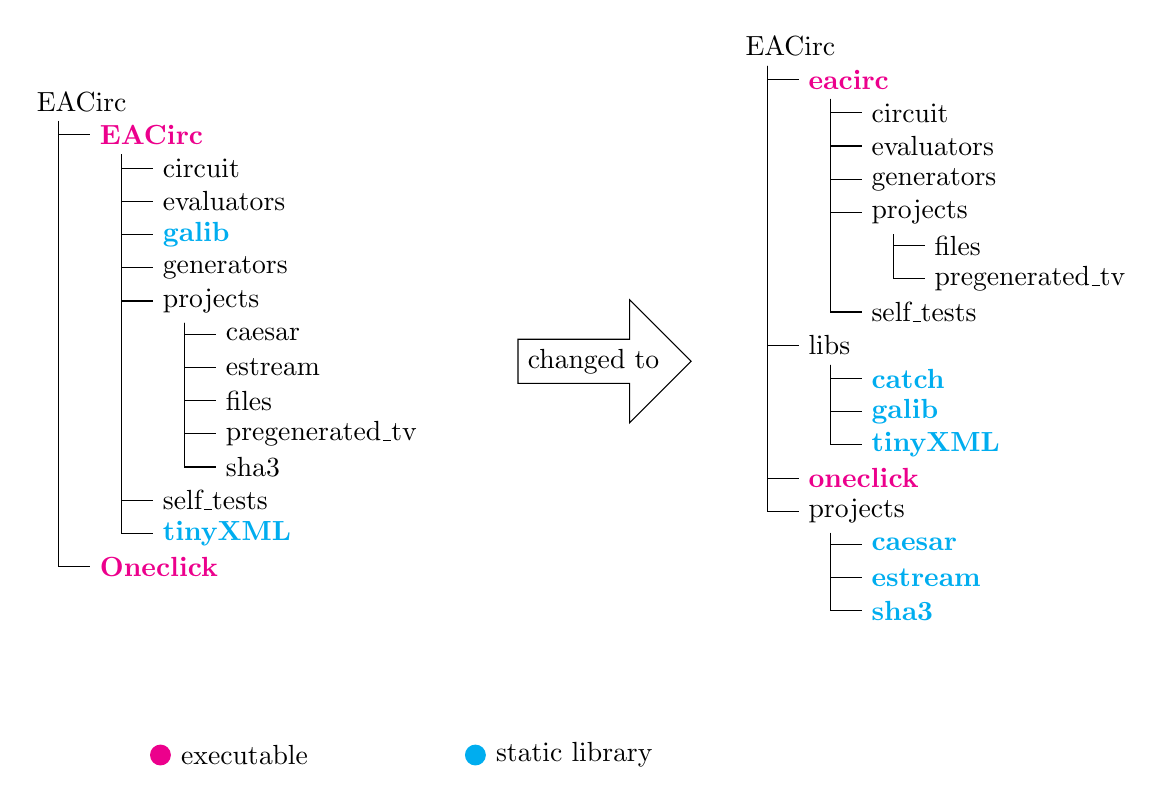
\begin{tikzpicture}[
grow via three points={one child at (0.8,-1.2em) and two children at (0.8,-1.2em) and (0.8,-2.4em)},
edge from parent path={($(\tikzparentnode\tikzparentanchor)+(.4cm,0pt)$) |- (\tikzchildnode\tikzchildanchor)},
growth parent anchor=west,
parent anchor=south west,
every child node/.style={anchor=west}
]
\node at (0,-2em) {EACirc}
	child { node [font=\bf,text=magenta] {EACirc}
		child { node {circuit} }
		child { node {evaluators} }
		child { node [font=\bf,text=cyan] {galib} }
		child { node {generators} }
		child { node {projects}
			child { node {caesar} }
			child { node {estream} }
			child { node {files} }
			child { node {pregenerated\_tv} }
			child { node {sha3} }
		}
		child [missing] {}
		child [missing] {}
		child [missing] {}
		child [missing] {}
		child [missing] {}
		child { node {self\_tests} }
		child { node [font=\bf,text=cyan] {tinyXML} }
	}
	child [missing] {}
	child [missing] {}
	child [missing] {}
	child [missing] {}
	child [missing] {}
	child [missing] {}
	child [missing] {}
	child [missing] {}
	child [missing] {}
	child [missing] {}
	child [missing] {}
	child [missing] {}
	child { node [font=\bf,text=magenta] {Oneclick}
	};
	
\node at (6.5, -4) [single arrow, draw, single arrow head extend=.5cm] {changed to};
		
\node at (9, 0) {EACirc}
	child { node [font=\bf,text=magenta] {eacirc}
		child { node {circuit} }
		child { node {evaluators} }
		child { node {generators} }
		child { node {projects}
			child { node {files} }
			child { node {pregenerated\_tv} }
		}
		child [missing] {}
		child [missing] {}
		child { node {self\_tests} }
	}
	child [missing] {}
	child [missing] {}
	child [missing] {}
	child [missing] {}
	child [missing] {}
	child [missing] {}
	child [missing] {}
	child { node {libs}
		child { node [font=\bf,text=cyan] {catch} }
		child { node [font=\bf,text=cyan] {galib} }
		child { node [font=\bf,text=cyan] {tinyXML} }
	}
	child [missing] {}
	child [missing] {}
	child [missing] {}
	child { node [font=\bf,text=magenta] {oneclick} }
	child { node {projects}
		child { node [font=\bf,text=cyan] {caesar} }
		child { node [font=\bf,text=cyan] {estream} }
		child { node [font=\bf,text=cyan] {sha3} }
	};
	
	\node at (1,-9) [scale=0.8,shape=circle,fill=magenta,label=right:executable] {};
	\node at (5,-9) [scale=0.8,shape=circle,fill=cyan,label=right:static library] {};
\end{tikzpicture}
	\caption{Old vs. new repository structure}
	\end{figure}
	
\noindent
The first and also the smallest change was to name all source folders with only small letters. Next the libraries from 3rd party providers \texttt{catch}, \texttt{galib}, and \texttt{tinyXML} were moved into the separate folder -- the \emph{libs} directory.

Then the so called \emph{projects} were isolated. A \emph{project} in EACirc terminology means a problem solving module. These \emph{projects} are \texttt{caesar}, \texttt{estream}, \texttt{sha3}, \texttt{files} and \texttt{pregenerated\_tv}. Since \texttt{files} and \texttt{pregenerated\_tv} are both just small modules consisting from only one source file, it would be impractical to isolated them. Whereas the big modules \texttt{caesar}, \texttt{estream}, and \texttt{sha3} were moved to the the separate folder called the \emph{projects} folder. Each of the isolated projects was remade to compile into a static library.\footnote{There is a plan to remake the projects to modules loaded dynamically at runtime. This would require to compile them separately into the dynamic libraries.}

The content od folders \texttt{eacirc} and \texttt{oneclick} is build into executables which are named accordingly to their corresponding folder. The \emph{projects} which are now compiled into the static libraries are now statically linked to the \texttt{eacirc} executable representing the EACirc tool as a whole. The \texttt{oneclick} executable is a supportive tool for automated task management developed by Ľubomír Obrátil. \cite{oneclick}

\section{The new build-system of EACirc}

The new build-system is written on the CMake platform. This platform allows to define custom options for generating the build. Here is a descriptive list of EACirc specific options:

\begin{description}
	\item[\texttt{BUILD\_ONECLICK}] enables building of Oneclick, the supportive tool for EACirc.
	\item[\texttt{BUILD\_CAESAR}] enables building of the Caesar project.
	\item[\texttt{BUILD\_ESTREAM}] enables building of the Estream project.
	\item[\texttt{BUILD\_SHA3}] enables building of the SHA-3 project.
	\item[\texttt{BUID\_CUDA}] enables to build the support for CUDA devices. This option is available only if the CUDA Toolkit \cite{cuda_toolkit} is installed on the build machine\footnote{A build machine is a physical or a virtual machine that is used to build the project.} and found by the CMake.
\end{description}

\noindent
Since the \emph{projects} are build into static libraries they must be linked to the \texttt{eacirc} executable at the compile time. This is done automatically when the option for the specific \emph{project} is enabled. In the figure \ref{fig:deps} are shown the dependencies of the all build targets.
	\begin{figure}[H]
	\begin{center}
		\includegraphics[width=.8\textwidth]{figures/deps}
	\end{center}
	\caption{EAcirc dependency graph}
	\label{fig:deps}
	\small
	The static libraries are shown in the rhombus. The executables have a house around them. The square represents an interface library.\footnote{Interface library does not need to be linked against. It consists only of header files.} The direction of the arrows represents that some build target depends on another one.
	\end{figure}

\noindent
The build-system is also version aware. The current version is stored in the \texttt{eacirc/Version.h} header file. The version corresponds to git commit hash \cite{git_book}. This means that for the correct build generation git tools must be properly installed on the build machine and found by CMake.\footnote{If git tools are installed and not found automatically by CMake then the path to git tools can be specified manually.}

The usage of CMake and the new options of building EACirc are explained in detail on the Github wiki project page under the Building EACirc section.

\section{Project settings for CUDA}

It is now much easier to set the project for CUDA support with CMake than with ordinal makefiles. When the CUDA Toolkit \cite{cuda_toolkit} is installed and automatically found by CMake\footnote{If CUDA Toolkit is installed on the build machine but not found by CMake automatically then the path to CUDA Toolkit can be specified manually.} then the option \texttt{BUILD\_CUDA} becomes available. If this option is enabled then the \texttt{eacirc} executable is build using Nvidia \cite{nvidia} \texttt{nvcc} compiler and the C preprocessor macro \texttt{CUDA} is defined causing that the executable will be runnable on CUDA capable devices. When writing a code for CUDA the preprocessor macro \texttt{CUDA} can be queried.

\printbibliography[heading=bibintoc]
\todo{Fix the autors of online resources}

\todo{Fix the titles in the bibliography to dislay big letters correctly.}

\todo{Cite Lobo's theses about oneclick and fix the source.}

\todo{Cite Martin Ukrop thesis in Introduction. What is EACirc?}

\end{document}